\chapter{Test af Implementation}

Som en del af udviklingsprocessen er der gennemført test af programmet. Testene er en undersøgelse, der kan give interessante informationer om programmets kvalitet. Softwaretest kan også give en objektiv og uafhængig vurdering af programmet. Test kan udføres som kørsel af programmet, med den hensigt at finde bugs eller andre fejl.

Til test af programmet anvendes forskellige testningsmetoder. Dette kapitel beskriver TDD, unit testing og manuel system test, som er metoder der benyttes til at teste implementeringen af løsningen.

\section{Systematisk Test af Program}
\label{sec:systematisk_test_af_program}

\subsection{Test Driven Development}
\label{sub:test_driven_development}

For at sikre at programmet er let at teste, er kernefunktionerne i programmet udviklet jævnfør softwareudviklingsprocessen \enquote{Test Driven Development}. I Test Driven Development (TDD) skrives unit tests af en metode, før selve implementeringen af funktionen. Denne udviklingsprocess sikrer, at nye funktionaliteter ikke ødelægger de forud eksisterende \cite{martin2006agile}. Programmøren tvinges også til at tænke på, hvordan metoden bruges ved kald. Det sikres hermed, at metoden er overskueligt konstrueret, således at den kan kaldes uden unødigt besvær. Et andet aspekt af TDD, er at testkoden tjener som dokumentation af den testede metodes funktionalitet. Tilgengæld riskeres et øget tidsforbrug, der dog muligvis kan fraskrives fejlfinding.

\subsection{Unit Testing i Microsoft Visual Studio}
\label{sub:unit_testing_i_microsoft_visual_studio}

Microsofts unit test framework for managed code er anvendt til unit testing. Frameworket kan teste \enquote{managed code}, som C\# falder ind under. Når tests er skrevet, kan Test Explorer i Visual Studio køre testene. Når testene er færdige, vil resultaterne blive præsenteret som failed tests, passed tests, not run tests og skipped tests \cite{msdn_unittest}.

Før der skrives unit tests, skal der oprettes et unit test projekt. Herefter kan der tilføjes klasser annoteret med \enquote{[TestClass]}. Inde i disse klasser, tilføjer man de metoder, annoteret med \enquote{[TestMethod]}, som skal køres. Et eksempel på en test metode, kan se i \cref{lst:test_notfound}.
Alle tests til systemet kan findes på CD'en der afleveres som bilag.

\begin{lstlisting}[label=lst:test_notfound, caption={Eksempel på testfunktion}]
  [TestMethod]
  public void ShouldThrowWhenNotFound()
  {
      var space = new WaterSpace(404404, 4.3, 5.4);
      try
      {
          var test = BoatDetector.BoatAt(space);
      }
      catch (KeyNotFoundException _)
      {
          return;
      }
      Assert.Fail("No exception was thrown.");
  }
\end{lstlisting}



\begin{figure}
  \centering
  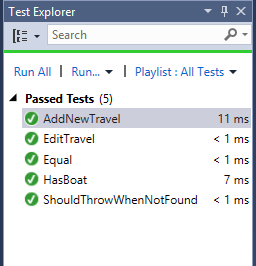
\includegraphics{test_explorer.png}
  \caption{Resultat af tests i Test Explorer i Visual Studio 2013}
  \label{fig:test_explorer}
\end{figure}

\section{System Test}
I dette afsnit vil der blevet testet hvorvidt udvalgte use cases kan udføres i programmet. De udvalgte use cases, er valgt på baggrund af deres evne til, at demonstrere funktionaliteten i programmet. Testene er opstillet således, at der startes med en hypotese omkring output ved forudbestemt input. Dernæst en gennemførsel af testen, og ud fra outputtet bedømmes resultatet som enten en \enquote{succes} eller \enquote{fejl}.

\textbf{Usercase 1: Et medlem ønsker at forlade sin plads i mere end 24 timer.}

Det antages at databasen tilfældigt generere et medlem ved navn "Johanne Hoffmann", båden "Den Usynkelige II", medlemsnummer 5 og passwordet "Johanne4395". Det antages også at Johanne vil rejse væk den 8/10-2014 og komme hjem den 18/10-2014.

Det forventes at med Johanne med sine login oplysninger kan opnå adgang til systemet, oprette sin rejse og få en bekræftigelse.
\begin{enumerate}
	\item Johanne starter programmet via .exe filen
	\item Johanne klikker på "Medlemslogin" og "Loginscreen" kommer dernæst frem og afventer input.
	\item Johanne indtaster sit medlemsnummer:"5" og password: "Johanne4395".
	\item Johanne klikker "Login" og forsidefanen kommer frem.
	\item Johanne navigere til brugeradministrationsfanen, og information omkring hende kommer frem.
	\item Johanne klikker på "Tilføj Ny Rejse" og "Tilføj rejse" bliver fremvist.
	\item Johanne vælger henholdsvis den 8/10-2014 og 18/10-2014.
	\item Johanne klikker OK, og kan nu se sin udrejse og hjemkomst i rejse feltet.
	\item Johanne kan nu logge ud eller tilgå andre funktioner i programmet.
\end{enumerate}

\textbf{Usercase 15: Havnefogeden vil gerne se hvornår et medlem vender tilbage til medlemmets plads.}

Det antages at Havnefogeden er genereret i databasen med medlemsnummer:"0" og passwordet:"havnefogedeVB1234". Det antages også at Havnefogede brugeren har skrive-tilladelse, som vil give ham fuld adgang. Det antages at dette sker efter foregående medlems interaktion med programmet, og det er det medlems rejse Havnefogeden er interesseret i. Det antages at det foregående medlem havde telefonnummeret: "22 95 41 87", og der er 3 medlemmer der hedder Johanne i databasen. Det antages at Havnefogeden har kun navnet "Johanne" og telefonnummeret "22 95 41 87"

\begin{enumerate}
	\item Havnefogeden kliker "Medlemslogin" og "Loginscreen" frem vises.
	\item Havnefogeden indtaster sit medlemsnummer:"0" og password:"havnefogedeVB1234".
	\item Havnefogeden kliker "Login" og forsidefanen kommer frem.
	\item Havnefogeden navigere til søgfanen.
	\item Havnefogeden indtaster navnet: "Johanne" hvor der kommer tre hits frem.
	\item Havnefogeden indtaster dernæst telefonnummeret: "22 95 41 87" og insnævre resultaterne til det rigtige medlem.
	\item Havnefogeden dobbeltklikker på medlemmet og får vist informationen omkring medlemmet "Johanne Hoffmann".
	\item Havnefogeden aflæser den ønskede data og er nu fri til at tilgå andre funktioner i programmet.
\end{enumerate}

% Dette er en test for det nuværende programs funktionalitet i forhold til de usescases, der er blevet opstillet for programmet.
% Ved Success forstås der at denne funktion er (delvis) mulig.
% Ved Implied forstås der at det er underforstået og/eller ude af programmets omfang.
% Ved Failure forstås der at denne funktion ikke er mulig i programmets nuværende stadie.
% \subsection{Medlemmer}


% \begin{enumerate}
	% \item{\bf{Medlem forlader sin plads i mere end 24 timer.}}
		% HANDLING: Medlemmet vælger "tilføj" under rejser, og vælger en afrejse og hjemkomst dato - Rejsen er nu gemt.
	  % \begin{enumerate}
			% \item Success -  a) Medlem melder til systemet et gyldigt tidspunkt for afrejse og hjemkomst.
			% \item Success -  b) Systemet melder til medlemmet at rejsen er registreret. 
			% \item Implied -  c) Systemet venter til efter tidspunktet for afrejse.
			% \item Failure -  d) Når pladsen tømmes, melder systemet at pladsen er fri.
	   % \end{enumerate}
			
	% \item{\bf{Alternativt medlem melder ikke afrejse til systemet.}}
	  % \begin{enumerate}
			% \item Failure -  aa) Systemet underetter havnefogeden om at en medlemsbåd har været væk fra havnen i mere end 24 timer
	   % \end{enumerate}
	   
	% \item{\bf{Alternativt medlem afrejser ikke på det meldte tidspunkt.}}
	  % \begin{enumerate}
			% \item Failure -  ba) Systemet underetter både havnefogeden samt medlemmet om uoverensstemmelsen.
	   % \end{enumerate}
	   
	% \item{\bf{Medlem vender tilbage til sin plads efter minimums 24 timers afrejse og der ligger en gæst på pladsen.}}
	  % \begin{enumerate}
			% \item Failure -  a) Systemet melder at pladsen er optaget.
	   % \end{enumerate}
	   
	% \item{\bf{Medlem vender ikke tilbage til sin plads på det meldte tidspunkt.}}
	  % \begin{enumerate}
			% \item Failure -  a) Systemet melder uoverensstemmelsen til havnefogeden
	   % \end{enumerate}

	% \item{\bf{Medlem ønsker at annullere en allerede anmeldt rejse.}}
		% HANDLING: Medlemmet logger ind og markere rejsen, dernæst klikker medlemmet på fjern - Rejsen er nu slettet
	  % \begin{enumerate}
			% \item Success -  a) Medlem vælger den pågældende rejse fra listen over registrerede rejser.
			% \item Success -  b) Medlem annullerer rejsen.
			% \item Success -  c) Systemet melder tilbage at rejsen er annulleret.
	   % \end{enumerate}

% \subsection{Gæster}
	% \item{\bf{Gæst er ankommet til havnen, og vil leje en plads.}}
		% HANDLING: Gæsten registrere sigselv i system og logger ind med udleveret chipkort. Gæsten kan nu se kortet over potentielt ledige pladser.
	  % \begin{enumerate}
			% \item Success -  a) Gæst registrere sig selv i systemet.
			% \item Failure -  b) Gæst benytter chipkortet til at logge ind.
			% \item Success -  c) Gæst finder oversigten over havnen og finder en ledig plads
			% \item Failure -  d) Gæst vælger den ledige plads og booker den.
			% \item Failure -  e) Gæst betaler for pladsen.
			% \item Failure -  f) Systemet melder til en at der er nye ankomne.
	   % \end{enumerate}
	   
	% \item{\bf{Alternativt: Gæsten finder ikke selv en plads.}}
	  % \begin{enumerate}
			% \item Success - a) Gæst registrere sig selv i systemet.
			% \item Failure - b) Gæst indtaster hans/hendes båds specifikationer.
			% \item Failure - c) Systemet returnerer en liste over pladser som vil passe hans behov.
			% \item Failure - d) Systemet videresender gæsten til betaling.
	   % \end{enumerate}

	% \item{\bf{Gæst vil se informationer om plads og betaling.}}
		% HANDLING: Gæsten indsætter chipkort og logger ind. I Brugeradministrations tabben vil information omkring gæsten samt hans båd og rejser befinde sig.
	  % \begin{enumerate}
			% \item Failure -  a) Gæst indsætter chipkort i automat.
			% \item Success -  b) systemet viser informationer vedrørende gæsten.
	   % \end{enumerate}
     
	% \item{\bf{Alternativt: Chipkort er bortkommet.}}
	  % \begin{enumerate}
			% \item Failure -  a) Gæster melder til systemet at chipkort er bortkommet.
			% \item Failure -  b) Systemet henviser gæsten til Havnefogeden.
	   % \end{enumerate}
     
	% \item{\bf{Gæst forlader havnen på eller før anmeldte afrejse tidspunkt.}}
	  % \begin{enumerate}
			% \item Failure -  a) Gæst aflever chipkort og får udleveret en kvittering.
			% \item Failure -  b) Gæst får returneret berettiget kapital.
	   % \end{enumerate}
    
	% \item{\bf{Alternativt: Gæst bliver liggende i havnen efter det anmeldte afrejse tidspunkt.}}
	  % \begin{enumerate}
			% \item Failure -  a) Systemet melder uoverensstemmelsen til havnefogeden.
			% \item Failure -  b) Chipkortet deaktiveres.
			% \item Failure -  c) Ved efterfølgende forsøg på brug af chipkort, henvendes der til havnefogeden.
	   % \end{enumerate}
			
	% \item{\bf{Gæst vil forlænge ophold.}}
		% HANDLING: Gæsten logger ind, og benytter ændre rejse funktionen. (Den opdateres ikke visuelt)
	  % \begin{enumerate}
			% \item Failure -  a) Gæst indsætter chipkort i automat.
			% \item Success -  b) Gæst melder ønskede ny afrejse dato til systemet.
			% \item Failure -  c) Systemet melder at den nye dato er registreret.
	   % \end{enumerate}
     
	% \item{\bf{Alternativt: Nye afrejse dato overlapper med medlemshjemkomst.}}
	  % \begin{enumerate}
			% \item Failure -  a) Systemet melder at datoerne overlapper, og foreslår ny plads.
	   % \end{enumerate}

% \subsection{Havnefoged}
	% \item{\bf{havnefogeden registrerer et medlemmets hjemkost.}}
		% HANDLING: Havnefogeden logger ind med hans login. Dernæst finder havnefogeden medlemmet og ændre datoen for hjemkomst i hans rejse.
	  % \begin{enumerate}
			% \item Implied -  a) Medlem meddeler tidlig hjemkomst til havnefogeden, for eksempel via telefon, mail eller lignende.
			% \item Success -  b) havnefogeden indtaster (ny) dato i systemet.
			% \item Success -  c) Systemet returnere at datoen er accepteret.
	   % \end{enumerate}

	% \item{\bf{Alternativt: En gæst har lejet pladsen for en længere periode.}}
	 % \begin{enumerate}
			% \item Failure -  a) Systemet foreslår en ny plads til gæsten.
			% \item Implied -  b) havnefogeden snakker med gæsten.
	   % \end{enumerate}
      
	% \item{\bf{havnefogeden vil gerne se hvilke pladser der er ledige.}}
		% HANDLING: Havnefogeden logger ind og klikker på kort tabben hvori der er et kort over havnen.
	  % \begin{enumerate}
			% \item Success -  a) havnefogeden åbner overbliksfunktionen i programmet.
			% \item Success -  b) havnefogeden kan nu se på et kort over havnen, hvilke pladser der er ledige.
	   % \end{enumerate}
      
	% \item{\bf{havnefogeden vil gerne se hvilke nye gæster der er ankommet indenfor et tidsrum.}}
	  % \begin{enumerate}
			% \item Failure -  a) havnefogeden åbner gæster funktionen i programmet.
			% \item Failure -  b) havnefogeden vælger det ønskede tidsrum.
			% \item Failure -  c) Programmet viser nye ankomne gæster fra det specificerede tidsrum.
	   % \end{enumerate}
  
	% \item{\bf{havnefogeden vil gerne se hvilke pladser der endnu ikke er betalt for.}}
	  % \begin{enumerate}
			% \item Failure -  a) havnefogeden åbner gæster funktionen i programmet.
			% \item Failure -  b) havnefogeden åbner ubetalte pladser.
			% \item Failure -  c) Programmet præsenterer listen af pladser, der endnu ikke er betalt for. Tiden for hvor lang tid pladsen har været ubetalt vises også.
	   % \end{enumerate}
	   
	% \item{\bf{havnefogeden vil gerne se hvornår et medlem vender tilbage til medlemmets plads.}}
	  % \begin{enumerate}
			% \item Success -  a) havnefogeden åbner medlems funktionen i programmet.
			% \item Success -  b) havnefogeden skriver i søgefeltet medlemmets navn eller medlemsnummer.
			% \item Success -  c) Programmet præsenterer en liste over matchende medlemmer.
			% \item Success -  d) havnefogeden vælger det søgte medlem.
			% \item Success -  e) Programmet viser alle kendte detaljer om medlemmet, herunder hvornår medlemmet forventes tilbage.
	   % \end{enumerate}
	   
	% \item{\bf{havnefogeden bliver advaret af en fejl ved en stander.}}
	  % \begin{enumerate}
			% \item Failure -  a) Uventet fejl opstår ved en stander på havnen, eller personen ved standeren trykker på hjælp.
			% \item Failure -  b) havnefogeden får besked om dette.
	   % \end{enumerate}

% \subsection{Andre}
	% \item{\bf{Automatisk arrangementsforslag.}}
	  % \begin{enumerate}
			% \item Failure -  a) Systemet melder på baggrund af aktiviteten i havnen, at det ville være en god dag for et arrangement.
			% \item Failure -  b) Et medlem af klubben ser denne melding, og foreslår et arrangement.
	   % \end{enumerate}
      
	% \item{\bf{Automatisk medlemstjek.}}
	  % \begin{enumerate}
			% \item Failure -  a) Systemet registrerer uoverensstemmelse med angivet rejseplan.
			% \item Failure -  b) Systemet notificerer havnefogeden omkring overensstemmelsen.
	   % \end{enumerate}
    
	% \item{\bf{Bestyrelsen eller havnefogeden vil se statistik over aktivitet i havnen.}}
	  % \begin{enumerate}
			% \item Failure -  a) Statistik funktionen åbnes og viser de ønskede statistikker.
	   % \end{enumerate}
			
	% \item{\bf{Kasser eller havnefogede vil tilføje ny båd til et medlem}}
	  % \begin{enumerate}
		% \item Success - a) havnefogeden logger ind i systemet med administrator rettigheder.
		% \item Success - b) Medlemmet bliver fundet via søge funktionen.
		% \item Success - c) havnefogeden tilføjer opretter en ny båd med pågældende information.
		% \item Success - d) Systemet melder tilbage at båden er registreret.
	   % \end{enumerate}

% \end{enumerate}

\section{Status på Program} 
\label{sec:status_p_program}

Dette afsnit har til formål at konkludere på programmets status. Der blev skrevet et program fordelt på 52 C\# kodefiler og 13 designfiler. En liste over disse filer, kan findes i \cref{cha:filliste}. 

Programmets hovedfunktioner såsom brugeradministration, visning af kort og søgefunktionaliteten fungererer efter hensigten, se \cref{sec:moduler}. Udover disse funktioner, mangler eller kan følgende funktioner forbedres. Chiplæseren ved login, er simuleret som et tekstfelt i brugergrænsefladen. Denne funktionalitet kan med fordel erstattes af en rigtig hardware chiplæser. En anden funktion der kan tilføjes til programmet er muligheden for at ændre brugertilladelserne ved programkørselstid. Derudover bliver hver bådplads sensor simuleret ved software. Det vil sige at sensoren kan styres fra programmet. En forbedring af denne funktionalitet, ville være at en rigtig hardware sensor bruges i stedet for den simulerede sensor.


%Programmet består af en brugergrænseflade, som inderholder fire faner med hver deres ansvarsområde. Den første fane er forsiden, som ikke indeholder funktionalitet, udover en beskrivelse af hvordan programmet bruges.


%Næste fane er kort funktionen, som viser et kort over en prædefineret havn. På fanen her er det muligt at se status på alle havnens pladser. Fra kortet er det også muligt at sende brugeren videre til brugeradministrationsfanen, ved at venstre klikke på en plads. Højere klikkes der på en plads vil pladsens oplysninger blive vist i et nyt vindue hvor det her er muligt at ændre pladsens egenskaber.

%Brugeradministrations fanen har til formål at vise informationer om en bruger, samt gøre det muligt at ændre i en brugers egenskaber. På siden er vist brugerens egenskaber og en liste af personens både. I listen er det muligt at vælge en båd og derved få vist bådens egenskaber.

